\documentclass[a4paper]{article}
\usepackage{listings}
\usepackage{pgf}
\usepackage[utf8]{inputenc}
\usepackage{verbatim}
\usepackage{titling}
\usepackage{booktabs}
\usepackage{enumitem}
\usepackage{qtree}
\usepackage{amssymb}
\usepackage{amsmath}
\usepackage{times}
\usepackage{dsfont}
\usepackage{titling}
\usepackage[a4paper,
bindingoffset=0.2in,
left=1in,
right=1in,
top=2in,
bottom=1in,
footskip=.25in]{geometry}
\usepackage{cite} %bibtex
\usepackage{pdfpages}

\pretitle{\begin{center}\linespread{1}}
  \posttitle{\end{center}\vspace{0.14cm}} 
\preauthor{\begin{center}\Large}
  \postauthor{\end{center}}

\setlength{\droptitle}{-10em}
\title { \Large{Seminario de Ciencias de la Computaci\'on B}\protect\\
  \large{Heurísticas de Optimización Combinatoria}\protect\\
  \large{Problema del k-\'arbol generador de peso m\'inimo\\con Optimización de Lobos Grises}}


\date{\normalsize{Martes, 25 de Abril, 2023.}}
\author{\normalsize{Profesor: Canek Peláez Valdés}\protect\\
  \normalsize{Autor: Xin Wen Zhang Liu}}\vspace{0.2cm}

\clearpage



\begin{document}
\allowdisplaybreaks
\maketitle

\subsection*{El problema del k \'arbol generador de peso m\'inimo}
La entrada de este problema es una gr\'afica completa no dirigida, sobre la cual se debe encotrar una subconjutno de k v\'ertices los cu\'ales generen un \'arbol de peso m\'inimo en la gr\'afica, entonces el resultado es un conjunto de $k$ v\'ertices y $k-1$ aristas dentro de la gr\'afica. Este problema es NP-duro, con una complejidad polinomial.


\subsection*{Optimizaci\'on del Lobo Gris / Grey Wolf Optimization}
Esta meta-heur\'istica fue inspirar por el comportamiento depredatorio de los lobos grises, y planteada Mirjalili
~\cite{MIRJALILI201446}. Propuesta como una nueva alternativa a la optimización por enjambre de
part\'iculas, este algoritmo simula el comportamiento depredatorio de los lobos gries , y su comportamiento jer\'arquico dentro de manadas.\\

Cada enjambre de lobos sigue una jerarqu\'ia social, como la que sigue
\begin{center}
  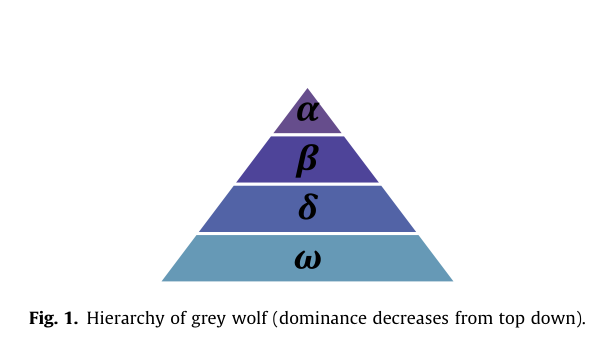
\includegraphics[width=\textwidth]{1682483544.png}
\end{center}

donde Alpha, Beta y Delta son las 3 mejores soluciones respectivamente, y todas las dem\'as son asignadas a los Omegas.

El modelo matem\'atico que representa a este algoritmo contiene las siguientes estapas
\begin{enumerate}
\item Acorralar a la presa
\item Caza
\item Atacar a la presa
  \end{enumerate}

  Los lobos acorrarlan y rodean a su presa cuando cazan, para modelar esto matem\'asticamente usamos
  la sigueinte ecuaci\'on
  \[\vec{D} = | \vec{C} \cdot \vec{X}_p(t) - \vec{X}(t)|\]
  \[\vec{X} (t+1) = \vec{X}_p (t) = \vec{A} \cdot \vec{D}\]
  donde $t$ respresenta la iteraci\'on actual y $\vec{A}, \vec{C}$ son vectores coeficiente. $\vec{X}_p$ es la posici\'on de la presa, de la cual no sabemos su paradero exacto, y es dependiente  al funci\'on de costo que se quiera usar. $\vec{X}$ indica la posici\'on del lobo en la iteraci\'on anterior.

Los vectores $\vec{A} $  y $\vec{C} $ son calculados de la siguente manera.
\[\vec{A} = 2 \vec{a} \cdot \vec{r}_1 -\vec{a}\]
\[\vec{C} = 2 \cdot \vec{r}_2\]
donde $\vec{a} $ es un componente lineal que decrese de 2 a 0, a lo largo de las iteraciones , y $r_1, r_2$ son n\'umeros aleatorios.

Los lobos son capaces de reconocer la unibaci\'on de su presa y rodearla. La caza es generalmente
guiada por el alpha. Sin embargo en un espacio de b\'usqueda abstracto es complicado saaber la
ubicac\'on de la presa (m\'inimo local). Para modelar este comportamiento de caza, asumimos que el alpha, beta y delta tiene el mayor conocimiento sobre de la ubicaci\'on de la presa. Por esot modificamos  a los dem\'as agentes a incluyendo a los omega a actualizar su ubicaci\'on en base a la de las 3
mejores soluciones. Para esto se utilizan las siguientes f\'ormulas.

\[\vec{D}_d = |\vec{C}_1\cdot  \vec{X}_d - \vec{X}|\]
\[\vec{X}_i = \vec{X}_d - \vec{A}_i \cdot \vec{D}_d\]
\[\vec{X}(t+1)  = \frac{\vec{X}_1 + \vec{X}_2 + \vec{X}_3}{3}\]


  
\section*{Diseño}

La gran parte de la heur\'istica se encuentra dentro del struct, GWO el cual se encarga de generar
conjuntos de v\'ertices en cada iteraci\'on de la evoluci\'on de los lobos, para generar los
\'arboles generadores de peso m\'inimo asociado. Para esto se implement\'o el algoritmo de Kruskal,
y sus funciones asociadas dentro de del struct Tree, y el cual igual regresa el pero asociado al
\'arbol el cu\'al es la evaluaci\'on de \"fitness\" de cada lobo.

Dentro del crate Tree, igual se encuentran los structs Edge y Vertex, que representan las aristas de
la gr\'afica y los v\'ertices respectivamente. Cada Edge est\'as compuesto de dos v\'ertices que
delimitan cada extremo de la arista, adem\'as de el peso asociado a esta. Los v\'ertices guardan el
valor de las coordenas en el palno xy, adem\'as de un identificador representado por un entero.

El struct Reader es el encargado, leer los puntos de un archivo de texto y crear V\'ertices que
guarden las coordenadas. 


\section*{Implementaci\'on}
El aplicar la heur\'istica al problema del k \'arbol generador de peso m\'inimo fue el proceso m\'as
tardado. La mayor\'ia del tiempo invertido en este proyecto fue hecho en la implementaci\'on de la
heur\'istica.

El primer paso fue investigar y comprender a fondo la idea general de \'esta para desp\'ues poder
aplicarlo a nuestro problema. La modificaci\'on del modelo para que se acoplara a lo necesario para
generar soluciones fue la parte m\'as 

 Cada lobo dentro de la manada tiene
asociado una soluci\'on del problema, y en cada iteraci\'on el conjunto de v\'ertice asociada a la
soluci\'on es modificada aleatoriamente, basado en la posici\'on de los lobos Alpha, Beta y Delta con las mejores soluciones. Cada lobo Omega actualiza su nueva posici\'on en base a estos, donde la
posici\'on es la que determina el nuevo v\'ertice que va a ser agregado para obtener el vecino.


La implementaci\'on de kruskal sigui\'o el algoritmo de union find ~\cite{unionFind} con path compression para una menor complejidad. Kruskal trabaja sobre una lista de aristas ordenaddas por su peso, y agarra en orden las aristas que no generen un ciclo dentro del \'arbol, esto hasta tener aritas que
conecten a todos los v\'ertices de la gr\'fica. Uno de los principales problemas de esta
parte de la implementaci\'on fue el refactorizar el c\'odigo para que aceptara valores flotantes. La primera implementaci\'on de este algoritmo fue usando HashMpas, lo que fue un error, ya que las
coordenadas y pesos de tipo flotante, hacen que muchas de las operaciones sean necesariamente implementadas a mano. 


Muchos de los problemas en rust surgen del tiempo de vida de vairables y de la posesi\'on de estas. Esto lleva a que un c\'odigo m\'as simple requiera de muchas m\'as copias de varibales para no tener
problemas con lo mencionado anteriormente, esto llea a programas menos optimizdos 
\section*{Experimentaci\'on y resultados}

Las soluciones generadas por la heur\'istica tardan en converger y mejorar los anteriores mientras
m\'as baja la evaluaci\'on del resutado anterior, teniendo un estacamiento al estar generando los
vecinos aleatorios en cada iteraci\'on.



La falta de experimentaci\'on llev\'o a un sistema menos predecible, y propenso a m\'inimos locales.
Por la manera en que lso lobos toman nuevas posiciones depu\'es de cada iteraci\'o hace que el rango de aleatoridad para ecoger nuevo v\'ertices sea pequeño, lo que lleva a que los agentes converjan a
un m\'inimo local y no haya una mayor exploraci\'on.

El promedio de la evaluaci\'on de los resultados encontrados por la heur\'istica sobre los puntos pasados por correo caen en el rango de $50 - 70$. 

El haber implementado la graficaci\'on de las soluciones ayud\'o el tipo de soluciones generadas y 


 Despu\'es de observar varias gr\'aficas generadas a lo largo de la ejecuci\'on, se not\'o que las gr\'aficas de las primeras iteraciones siempre segu\'ian una forma m\'as esparcida
en el espacio de b\'usqueda, sin embargo al continuar con la ejecuc\'i\'on y al ir mejorando las
soluciones, las gr\'aficas terminaban teniendo una forma m\'as compacta a las iniciales. Sin embargo, por


Para solucionar esto se implement\'o una manera diferente de seleccionar los vecinos en cada iteraci\'on. Primero se busca el centro geom\'etrico de la gr\'aafica y a partir de esto se compara con
todos los puntos en la soluc\'on anterior y se encuentra al m\'as alejado, el cual va a ser el que
sea modificado para encontrar una soluci\'on vecina. Despu\'es de esto se busca un v\'ertice al azar
el cual tenga una distancia al centro geom\'etrico menor del v\'ertice que se elimin\'o. De esta
manera cada agente llega exaustivamente a un m\'inimo local.

Con esto se logr\'o que las soluciones encontradas bajaran de un peso de $50-70$ para el conjunto
original de puntos, a poder encontrar la soluci\'on \'optima de 30.

\section*{Conclusiones}
La planeaci\'on en este caso podr\'ia haberse visto avanzada con la implementaci\'on del programa,
ya que crea dudas reales que aplican al c\'odigo del programa y nos hace preguntarnos de la mejor
manera de implementar lo requerido .

La experimentaci\'on no s\'olo conlleva a encontrar mejores resutlados sino igual a mejorar el
c\'odigo para que la calidad de los resultados sea cada vez m\'as alta. Es por esto que

Por la falta de tiempo la optimización del sistema fue escaza, por lo que el experimentar fue m\'as
tardado de lo normal.


\bibliography{citations}{}
\bibliographystyle{plain}
\end{document}